\documentclass[a4paper, 8pt]{memoir}

\usepackage{fontspec}
\usepackage{verbatim}
\usepackage[version=3]{mhchem}
\usepackage{chemfig}
\usepackage{rotating}

%This package goes last.
\usepackage{hyperref}
\setmainfont{FreeSerif}

\newcommand*{\el}{e$^-$}

\begin{document}
\chapter{The History of the Discovery of the Atom}
\section{Development of the Structure of the Atom}
\begin{tabular}{|c||p{2in}|p{2in}|}
\hline
Dalton & Sphere & All things made of tiny spheres \\ \hline
J.J. Thompson & Raisun Bun/Plum Pudding & Positive pudding with negative cherries \\ \hline
Rutherford & Nucleus with electron cloud & Protons \& neutrons in nucleus, \newline in an electron cloud \\ \hline
Bohr & Electrons on orbitals & Electrons on specific orbitals (planetary) \\ \hline
Einstein, Planck, Heisenberg & Quantum Mechanics & Areas of probability of electrons \\ \hline
\end{tabular}
QM just has yet to be disproved...
\section{Discovery of Subatomic Particles}
\subsection{The electron: first to be found}
\subsubsection{Faraday}
Produces the first cathode ray tube. It has two electrodes and is made of glass. It contains a near-vacuum. When powered on, the tube glowed green.
\subsubsection{Crookes}
Investigated properties of cathode rays.
\begin{itemize}
\item massive
\item has energy
\item travels in a straight line
\end{itemize}
\subsubsection{J.J. Thompson}
Found the electron.
\begin{enumerate}
\item Putting the tube between a positively charged plate and a negatively charged one, the glow was repelled by the negative glow. Hence the glow is negatively charged.
\item Surrounding the tube with a magnet (such as a horseshoe), the glow was affected. Hence the glow is electrical in nature.
\item By putting magnets of various strengths at various places and deflecting the ray, he calculated the charge to mass ratio of an electron (not to be memorized).
\item After changing the gas in the tube, the same ratio was calculated.
\item After changing the metals in the electrodes, the same ratio was calculated.
\end{enumerate}
\subsection{The Proton}
\subsubsection{Goldstein, 1886}
Using a \emph{canal ray tube}, a modified cathode ray tube, Goldstein identified the positive particle in the atom. Its mass varied with the residual gas. When \emph{hydrogen} was the residual gas, the least massive particle was produced. This particle was accepted as the \emph{fundamental positive particle of matter}.

The instrument was shaped like a flat (♭). One electrode was placed at the top of the round, and another at the lower junction. Electrons would be able to complete the circuit, but protons would be too massive and would be thrown into the upper chamber by their momentum.
\subsection{The Neutron}
Proposed to exist in 1920.
Chadwick discovered it in 1932.
\section{Radiation}
Henri Becquerel discovered radiation.
Rutherford discovered alpha and beta radiation.
\chapter{Balancing Nuclear Equations}
\begin{tabular}{|c|c|c|c|c|}
\hline
Name & Atomic Mass & \# of protons & Greek Letter & Symbol \\ \hline
Alpha & 4 & 2 & α & \ce{^{4}_{2}α} \\ \hline
Beta & 0 & -1 & β & \ce{^{0}_{-1}β} \\ \hline
Gamma & 0 & 0 & γ & \ce{^{0}_{0}γ} \\ \hline
\end{tabular}
\begin{itemize}
\item U loses 2 alpha particles and 3 beta particles

\ce{^{238}_{92}U -> 2^{4}_{2}α + 3^{0}_{-1}β + ^{230}_{91}Pa}
\item Ra loses 100 gamma particles

\ce{^{226}_{88}Ra -> 100^{0}_{0}γ + ^{226}_{88}Ra}
\end{itemize}
\chapter{Rutherford's Gold Foil Experiment}
α particles were shot from lead in a box through a slit in a circle of detecting screen at the sheet of gold foil one atom thick inside. Most particles penetrated but some were deflected or reflected. He predicted that there was something small and dense within the atom, rather than the atom's being a positive pudding.
\chapter{Bohr's Colour Spectrum}
It only works for hydrogen. 

When an electron absorbs energy, it leaps to a higher orbital. When the source of energy is cut, the electron emits its energy as a wavelength, such as light, and the electron retreats to a lower orbital.

For hydrogen, the spectrum has 4 lines.

\begin{tabular}{|c|c|}
\hline
Colour & Jump \\ \hline
Red & 3 -> 2 \\ \hline
Blue & 4 -> 2 \\ \hline
Violet 1 & 5 -> 2 \\ \hline
Violet 2 & 6 -> 2 \\ \hline
\end{tabular}
\chapter{Electromagnetic Radiation}
Light travels through space in a wave that is composed of two perpendicular components, an electric component and a magnetic component.
\begin{description}
\item[wavelength] distance between two peaks of a wave (metres)
\item[frequency] number of cycles past a point per second (Hz or $s^{-1}$)
\end{description}
\begin{align}
c &= 3.00 \times 10^{8} ms^{-1} \\
v &= \lambda f
\end{align}
The velocity of ER in a vacuum is constant.

\emph{Planck} (1900) began the quantum revolution with a surprising interpretation of the results of a study of the light emitted by hot objects. He theorized that the energies of the oscillating atoms in the heated solid were multiples of a small quantity of energy. \emph{Energy is not continuous.}
\begin{align}
h &= 6.626 \times 10^{-34} Js \\
E &= hf
\end{align}
\section{Continuous spectrum}
When white light is passed through a prism, it produces a continuos spectrum that represents all possible frequencies or energies of light in the visible spectrum.
\begin{center}
\begin{tabular}{|c|c|}
\hline
Frequency & Colour \\ \hline
400nm & violet \\ \hline
 & indigo \\ \hline
500nm & blue \\ \hline
 & green \\ \hline
600nm & yellow \\ \hline
 & orange \\ \hline
700nm & red \\ \hline
\end{tabular}
\end{center}
\section{Line Spectrum}
When light from a single element is passed through a prism, the spectrum consists of only a few frequencies.

The H$_2$ spectrum consists of violet 2, violet 1, blue-green, and red. All hydrogen atoms exhibit the same spectra, with bands of light with the exact same wavelengths, frequencies, and energies.
\section{Wave-particle duality theory}
De Broglie (1924) suggested that small particles like electrons behave not only like solid particles but also like waves. Thus they disobey classical laws of physics and are governed by quantum mechanics, the newer set of laws.
\begin{align}
\lambda &= \frac{h}{mv} 
%m &= \frac{Js}{kg\cdot{}m\cdot{}s^{-1}} \\
%J &= m\cdot{}s^{-1}kg\cdot{}m\cdot{}s^{-1} \\
%&= kg\cdot{}m^{2}\cdot{}s^{-2} \\
\end{align}
where m is the mass of an electron (to be given), v is velocity.
\section{Motion of waves}
Schrodinger (1926) used quantum mechanics to develop an atomic model based on the wave nature of electron. From his equation that explained the motion of the wave came four \emph{quantum numbers} that described the electronic structure of the atom.
\section{Quantized (discrete) nature of light emitted by a hot solid}
Einstein (1905) pointed out the above, and called these packets quanta.
\begin{align}
E &= \frac{hc}{\lambda}
\end{align}
\section{Heisenberg's Uncertainty Principle}
\begin{quote}
The more precisely position is determined, the less momentum is known in the instant, and vice versa
\end{quote}
Mathematically showed that there are definite limits to our ability to know both the position and the momentum of a particle. Because it is impossible to know where an electron is, we can only describe electrons through location probability fields.
\section{Bohr model of the atom}
\begin{enumerate}
\item The electrons in an atom revolve about the nucleus in fixed orbits.
\item Each orbit has an energy value that electrons in the orbit must have.
\item Each atom has certain allowed orbits and energy levels.
\item Electrons can move from a lower energy level to a higher energy level be absorbing the exact difference in energy. The energy of an electron is quantized: it can only have certain allowed values of energy.
\item To move from a higher energy level to a lower one, the electron must lose energy equal to the difference in energies. The energy is emitted as electromagnetic radiation of different frequencies.
\item By measuring the frequency of light emitted in the spectrum of an atom, we can calculate the energy difference between two orbits.
\end{enumerate}
Bohr equation for the energy of an electron (orbital) in hydrogen.
\begin{align}
k &= 2.18 \times 10^{-18} J \\
E &= \frac{-k}{n^{2}}
\end{align}
where n is the orbit number.

Again, Bohr's model only worked for hydrogen.
\begin{align}
E_\textit{total} &= E_\textit{initial orbital} - E_\textit{final orbital}
\end{align}
\chapter{Isotomes and Radioisotopes}
\begin{description}
\item[isotope] Element with same \# of protons but different \# of neutrons e.g. \ce{^{1}H} (hydrogen), \ce{^{2}H} (deuterium), \ce{^{3}H} (tritium), \ce{^{2}H_{2}O} (deuterium (heavy water))
\item[radioisotope] Isotope that emits radioactivity. All elements have 1+ unstable isotopes that attain a stabler state by losing energy called \emph{radioactivity}.
\end{description}
\section{\ce{^{14}C} dating}
\begin{itemize}
\item A neutron bumped from an atom by cosmic rays becomes energetic and bombards \ce{^{14}N} in the upper atmosphere
\item This forms \ce{^{14}C} as a hydrogen atom (a proton (and an electron?)) is removed
\item \ce{^{14}C} is used to determine the age of \emph{organic materials}
\item \ce{^{14}C} has a half-life of 5700 years
\item \ce{^{14}C} combines with upper atmosphere oxygen and forms small amounts of \ce{CO_{2}}, which is absorbed by plants during photosynthesis. Thus plant and animal tissue contains \ce{^{14}C}.
\item On death, \ce{^{14}C} intake stops and amount of \ce{^{14}C} decreases whilst \ce{^{12}C} increases.
\item By comparing \ce{^{14}C} of organic material with \ce{^{14}C} in living organism, age can be determined.
\end{itemize}
\chapter{Relative Atomic Mass}
\begin{align}
RAM = (AM\times{}\%Abundance)+(AM\times{}\%Abundance)+\dotsc
\end{align}
RAM is in amu (atomic mass units).
\chapter{Quantum Numbers : The Quantum Mechanical Model}
\section{n}
Defines the \emph{size} of an electron wave: its extent from the nucleus. Has an allowed range of $1,2,3,\dotsc$. Same as the row number.
\begin{enumerate}
\item first energy shell; first energey level; K-shell
\item L-shell
\item M-shell
\end{enumerate}
\section{l}
Defines the \emph{shape}. Range of [0, n-1].
\begin{tabular}{|c|c|}
\hline
l & Orbital shape \\ \hline
0 & s \\ \hline
1 & p \\ \hline
2 & d \\ \hline
3 & f \\ \hline
\end{tabular}
\section{m(agnetic)}
Represents \emph{orientation in space} of orbital. Range of [-L, +L].
\section{s(pin), $m_s$}
Defines \emph{spin} of electron. For purposes of the course, it may only be ±½.
\section{Principles of Electron Configuration}
\begin{description}
\item[Pauli exclusion principle] No 2 electrons in one atom can have the same four quantum numbers. Since s has only two values, each orbital may only have 2 electrons.
\item[Aufbau Principle] An energy sublevel must be filled before moving on to the next higher sublevel.
\item[Hund's Rule] If there are several orbitals at the same energy, one electron is placed into each before a second one is added.
\item[Don't forget] to draw the arrow, label it "Energy", and write the element symbol.
\end{description}
\begin{center}
\begin{tabular}{|c|c|c|c|c|}
\hline
Element & n & l & m & s \\ \hline
Be & 2 & 0 & 0 & -½ \\ \hline
Nd & 4 & 3 & 0 & ½ \\ \hline
K & 4 & 0 & 0 & ½ \\ \hline
\end{tabular}
\end{center}
\chapter{Dmitri Mendeleev}
Chemists of the day tried to organize elements into useful patterns. The First International Congress was held in Karlsruhe, Germany in 1850. Italian chemist Cannizaro differentiated atomic and molecular mass in a paper. Afterwards, attempts were made to organize elements by atomic mass. English chemist Newland found that for lighter elements, properties repeated themselves in each group of seven. In 1854, Newland announced his discovery as the Law of Octaves, but failed to fit the heavier elements into the pattern.

Mendeleev noted that when lithium, magnesium, boron, carbon, oxygen, and chlorine were arranged by atomic mass, their valences were
\begin{center}
1,2,3,4,3,2,1
\end{center}
The pattern repeated itself when the next seven were arranged by atomic mass. Mendeleev arranged the 63 then-known elements in a table so that elements with the same valence were in the same row (these are today in the same column). Since the elements showed a periodic variation in valence, he called it a \emph{Periodic Table of the Elements}. It looked like \href{http://bit.ly/15ceGf5}{this}.

Mendeleev left gaps where elements with the right valences had not been discovered. He predicted that they would be discovered, and also he predicted their physical and chemical properties. 

The elements in Group VIII (noble gases) were excluded from the periodic table because they were so unreactive that they were unknown until the work of William Ramsey. Mendeleev missed the Nobel Prize in Chemistry in 1906 by one vote.
\chapter{Periodic Trends}
\begin{description}
\item[Atomic Radius] As you move left, the pull of the nucleus weakens, and the atom grows. As you move down, an orbital shell is added and the atom grows.
\item[First Ionization Energy (energy needed to remove outermost electron)] The stronger the pull of the nucleus, the more energy is needed. So IE increases as you go right, opposite atomic radius. As you go up, AR goes down, and IE goes up.
\item[Electron Affinity (energy released when electron is added to neutral atom)] The greater the pull of the nucleus, the larger the release of energy. So EA increases as you go right. As you go up, AR goes down, and EA goes up.
\item[Electronegativity (tendency of an atom to attract electrons)] Immeasurable, a relative value. As AR goes down, EN goes up.
\item[Reactivity] For nonmetals, it goes up towards the upper-right (\ce{Cl}). For metals, it goes up towards the bottom-left (\ce{Fr}).
\end{description}

In short: 
\begin{itemize}
\item ER, IE, EN, nonmetal reactivity increase towards the top right. 
\item AR and metal reactivity increase towards the bottom left.
\end{itemize}

\chapter{First Ionization Energy, Electron Affinity, Electronegativity}
Metals have a higher first ionization energy than electron affinity and so they lose electrons. Nonmetals have a higher elctron affinity than first ionization energy and so they gain electrons.

\chemfig{\lewis{0.,Na}\chemrel{->}\lewis{0:2:4.6:,Cl}}

\chemfig{\lewis{0:2:4:6:,Cl}\lewis{0:2:6:,Cl}}

The above ions have a \emph{shared pair}. It can be notated as below:

\chemfig{\lewis{2:4:6:,Cl}-\lewis{0:2:6:,Cl}}

\section{Electronegativity}
If the difference between two elements' electronegativities $>=$ 1.7, they will form an ionic bond \\
If $\Delta{}EN < 1.7$, covalent

\begin{align*}
C_{EN}-H_{EN} &= 2.5-2.1 \\
&= 0.4 \\
&< 1.7
\end{align*}
Therefore, $CH_4$ is covalent.

\begin{align*}
Cl_{EN} - H_{EN} &= 3 - 2.1 \\
&= 0.9 \\
&< 1.7
\end{align*}

And yet, \emph{HCl is ionic.} Consider the way it reacts with $H_2O$.
\chapter{Bonding}
\begin{description}
\item[potential energy] energy available to do something

\ce{Na_{(g)} -> Na^+_{(g)} + e^-} \\
\ce{Cl_{(g)} + e^- -> Cl^-_{(g)}} 

Note that \emph{ions are gaseous}.

The first ionization energy of sodium is 495.4 kJ mol$^{-1}$ (absorbed). The electron affinity of chlorine is -348.8 kJ mol$^{-1}$ (emitted). Adding gives us 146.6 kJ mol$^{-1}$.

This tells us that potential energy must increase for the reaction to happen. This shows that just ionizing the elements is not enough to form compounds.

\item[lattice energy] measure of attraction between ions (something about enthalpy)

NaCl has a lattice energy of -787 kJ mol$^{-1}$.

\begin{align*}
FIE + EA + LE &= 495.4 - 348.8 - 787 \\
&= -640.4 kJ mol^{-1}
\end{align*}

Potential energy decreased in the reaction, so it is stable.

\item[Coulomb's Law] \begin{equation}
E_{lattice} = \frac{q_1 q_2}{k r}
\end{equation}
Where:
\begin{itemize}
\item $q_n$ = charge of the nth ion
\item k = Coulomb's constant
\item r = ionic radius
\end{itemize}

Na$^+$ is smaller than Cl$^-$ because when Na loses an electron, it has lost a whole energy level.

K$^+$ is also smaller than Cl$^-$ because it has more protons and electrons and is able to pull them in more tightly than chlorine (which has more electrons than protons).

Let $r_1$ be the ionic radius of NaCl, and $r_2$ be the ionic radius of KCl. Then,

\begin{align*}
E_{NaCl} &= \frac{(+1)(-1)}{kr_1} \\
E_{KCl} &= \frac{(+1)(-1)}{kr_2} \\
\end{align*}

Na$^+$ is smaller than K$^+$, so $r_1$ is less than $r_2$. Then, $E_{NaCl}$ is less than $E_{KCl}$.

Therefore $E_{NaCl}$ is more stable. Remember, energy means the chance of stuff happening, so less energy (more potential energy used; more energy used) means more stability. Also remember that in the above example, the fraction is negative, so a larger denominator means in fact a larger energy value.
\end{description}

Forming an ionic compound:

\begin{tabular}{|l|l|}
\hline
\ce{Na_{(s)} + ½Cl_{2(g)}} & +107.8 kJ mol$^{-1}$ : Sublimation Energy \\
\ce{Na_{(g)} + ½Cl_{2(g)}} & +121.3 kJ mol$^{-1}$ : Energy to isolate 1 atom \\
\ce{Na_{(g)} + Cl_{(g)}} & +495.4 kJ mol$^{-1}$ : First Ionization Energy (Sodium) \\
& -348.8 kJ mol$^{-1}$ : Electron Affinity (Chlorine) \\ 
\ce{Na_{(g)}^{+} + Cl_{(g)}^{-}}  & -787 kJ mol$^{-1}$ : Lattice Energy (NaCl) \\ \hline
\ce{NaCl_{(s)}} & -411.3 kJ mol$^{-1}$ \\ \hline
\end{tabular}

\ce{Na_{(s)} + ½Cl_{2(g)} -> NaCl_{(s)} - $411.3$ kJ mol^{-1}}

-411.3 kJ mol$^{-1}$ is the standard heat/enthalpy of formation.

$\Delta H^{\circ}_{f} = -411.3 kJ mol^{-1}$


\section{Covalent Molecules}
For covalent molecules, the ionic radius is still the distance between their nuclei. Unlike ionic compounds, the outer orbits of the atoms \emph{overlap}, creating a decentralized zone where electrons can travel between the atoms.\\

The potential energy of as two hydrogen nuclei get farther apart:
\begin{itemize}
\item At first it is above the potential energy of one hydrogen. It is steeply falling.
\item It drops below that of one hydrogen. It is starting to flatten
\item It is at the absolute minimum, its most stable. Convalent bonding occurs.
\item Once the bond is formed, pulling the atoms apart causes potential energy begins to rise steeply again.
\item Eventually, though, it starts to flatten again. The original potential energy of one hydrogen is a horizontal asymptote.
\end{itemize}

If you can't imagine it, it's kind of like this:\\
\rotatebox{-90}{\Huge ¸}

Potential energy is the vertical axis. Nucleic distance is the horizontal axis.

\chapter{Lewis Structure}
The example is \ce{[FI_{4}]^{-}}.
\begin{enumerate}
\item Atom orientation: put the least electronegative atom in the centre \\
Flourine has an electronegativity of 4.1 which is greater than iodine's 2.2. So in the centre goes iodine.
\item Count the total valence electrons. Add or subtract accordingly for charged compounds  \\
Iodine has 7, and four flourines have 28. This compound is negatively-charged, so there is one extra electron.  \\
A total of 7+28+1 = 36 \el.
\item Connect everything with single bonds \\
\chemfig{F-I(-[0]F)(-[2]F)(-[6]F)} \\
Each single bond is 2 electrons. So now we have 36 \el - 4$\times$2 \el = 36 \el - 8 \el = 28 \el.
\item Fulfill the octet rule in the surrounding atoms \\
\chemfig{\lewis{2:4:6:,F}-I(-[0]\lewis{0:2:6:,F})(-[2]\lewis{0:4:2:,F})(-[6]\lewis{0:4:6:,F})} \\
Now we have 28 \el - 24 \el = 4 \el.
\item And we plunk the remainder onto the central atom. \\
\chemfig{\lewis{2:4:6:,F}-\lewis{1:5:,I}(-[0]\lewis{0:2:6:,F})(-[2]\lewis{0:4:2:,F})(-[6]\lewis{0:4:6:,F})}
\end{enumerate}

Et voilà! Note that iodine has 12 outer electrons, which is OK because iodine's outer orbital has room for 18 (look at its row in the periodic table).

\begin{description}
\item[bond order] Number of electron pairs shared by atoms
This is a measure of the electron density of a bond. The denser, the stronger the attraction forces between the nuclei, and the shroter the bond length.
\item[formal charge] Theoretical charge of each atom in a compound

FC= Number of valence \el - Number of bonds - Number of unbonded \el

\item[preferred structure] Chemical structure that has the most neutral atoms (the charges are the most evenly distributed) \\
\chemfig{H-\lewis{2:6:,O}-S\rlap{$^{+2}$}(-[2]\lewis{0:2:4:,O\rlap{$^{-1}$}})(-[6]\lewis{0:4:6:,O\rlap{$^{-1}$}})-\lewis{2:6:,O}-H}

Is \emph{less} preferable than

\chemfig{H-\lewis{2:6:,O}-S(=[2]\lewis{0:4:,O})(=[6]\lewis{0:4:,O})-\lewis{2:6:,O}-H}

\section{Exceptions!}
B and Be need not satisfy the octet rule.

\chemfig{\lewis{2:4:6:,Cl\rlap{$^{0}$}}-B\rlap{$^{0}$}(-[6]\lewis{0:4:6:, Cl\rlap{$^{0}$}})-\lewis{0:2:6:,Cl\rlap{$^{0}$}}}

Even though the octet rule is not satisfied, the above is correct.

\chemfig{\lewis{2:6:,Cl\rlap{$^{+}$}}=B\rlap{$^{-}$}(-[6]\lewis{0:4:6:, Cl})-\lewis{0:2:6:,Cl}}

There's no way the more electronegative Cl would have a more positive charge than B. So this form is wrong.
\end{description}

\chapter{Resonance}
Resonance refers to bonds that are shorter than they should be. \\

\schemestart
\chemleft[\chemfig{H-C(=[1]\lewis{2:6:,O})(-[7]\lewis{0:2:6:,O})}\chemright]$^{-}$ \arrow{<->} \chemleft[\chemfig{H-C(=[7]\lewis{2:6:,O})(-[1]\lewis{0:2:6:,O})}\chemright]$^{-}$
\schemestop

Both of the above are pluasible structures. \\

Those bonds that alternate are shorter than they should be. They're actually both halfway between single and double bond length. They're like hybrid bonds. \\

Bond order = $\frac{\text{Number of bonds}}{\text{Number of orientations}}$ \\

Hence we say these bonds have bond orders of $\frac{3}{2}$ or $1\frac{1}{2}$. \\

\chapter{Structure of Crystalline Solids}
\begin{description}
\item[crystal lattice] repeating array of particles
\item[unit cell] repeating unit
\item[lattice point] points within unit cell at the centre of each particle
\end{description}

There are some twelve shapes, but the two you will need to know are these cubic lattices (the lattice points form right angles, and the lengths of the unit cells are all equal):
\begin{description}
\item[Face-centred cubic] Point on the centre of every face \\
There are 8 corner particles and 6 face particles. \\
\begin{align*}
\text{8 corners} + \text{6 faces} &= 8(\frac{1}{8}) + 6(\frac{1}{2})
&= 1 + 3
&= \text{4 particles}
\end{align*}
\item[Body-centred cubic] Point in the centre of the cube \\
There are 8 corner particles and 1 central particle. \\
\begin{align*}
\text{8 corners} + \text{1 centre} &= 8(\frac{1}{8}) + 1(1)
&= 1 + 1
&= \text{2 particles}
\end{align*}
\end{description}

Look at \href{http://bit.ly/101SXqL}{this} \\

And then table salt is special. NaCl has alternating Na and Cl along every edge, through every face and corner. \\
The corner and face particles are Cl.
\begin{align*}
\text{8 corners} + \text{6 faces} &= 8(\frac{1}{8}) + 6(\frac{1}{2})
&= 1 + 3
&= 4 Cl^{-}
\end{align*}
The edge and central particles are Na.
\begin{align*}
\text{12 edges} + \text{1 centre} &= 12(\frac{1}{4}) + 1(1)
&= 3 + 1
&= 4 Na^{-}
\end{align*}

To recap:
\begin{itemize}
\item Corner is worth $\frac{1}{8}$
\item Edge is worth $\frac{1}{4}$
\item Face is worth $\frac{1}{2}$
\item Centre is worth 1
\end{itemize}

\chapter{VSEPR, shape, polarity}
\begin{description}
\item[Valence shell electorn pair repulsion] electrons in the valence shell move as far as part as possible to minimize repulsion
\item[electron domain] a region occupied to valence electorn pairs. Can be bonding or non-bonding
\item[bonding domain] space occupied by shared electrons i.e. a bond, regardless of order
\item[non-bonding domain] space occupied by lone pair
\end{description}
\section{Electron Geometry}
Varies with the number of electron domains.
\subsection {Planar EGs}
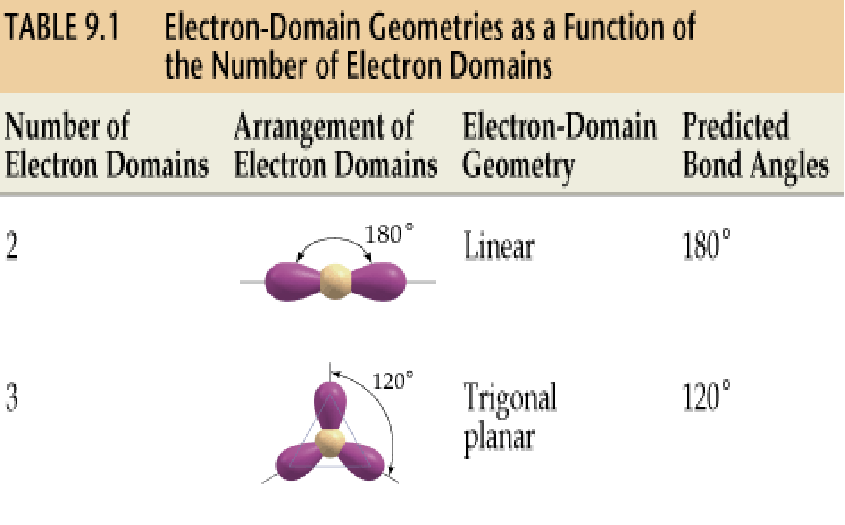
\includegraphics[scale=0.4]{planarElectronGeos}
\subsection {3-D EGs}
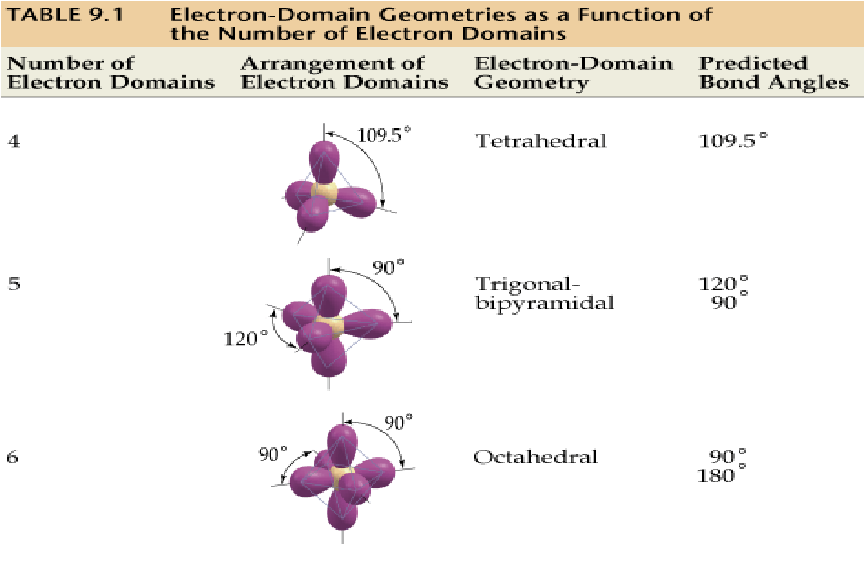
\includegraphics[scale=0.4]{3dElectronGeos}
\section{Molecular Geometry}
Varies with the number of bonding and non-bonding domains. \\
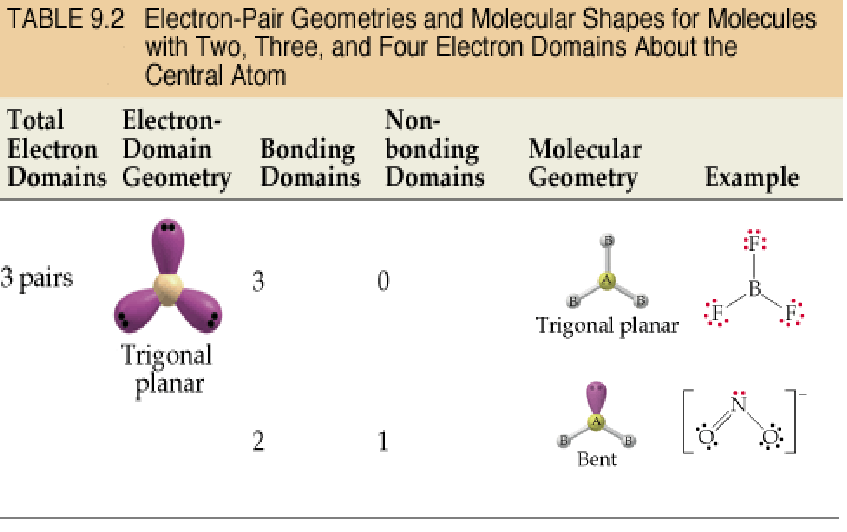
\includegraphics[scale=0.4]{molgeo3} \\
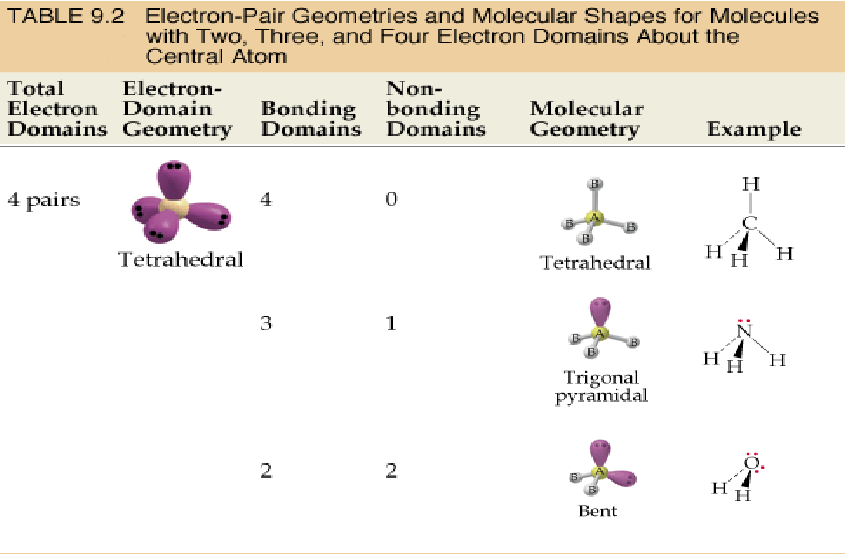
\includegraphics[scale=0.4]{molgeo4} \\
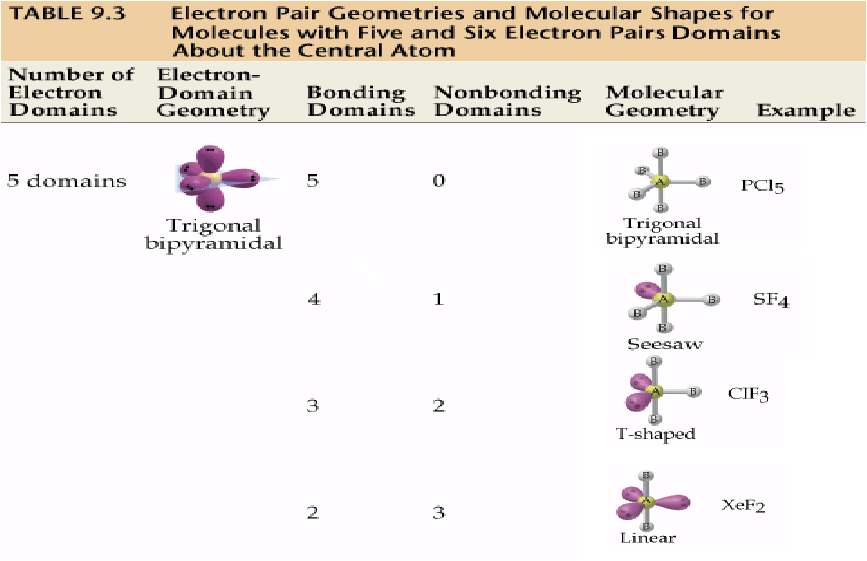
\includegraphics[scale=0.4]{molgeo5} \\
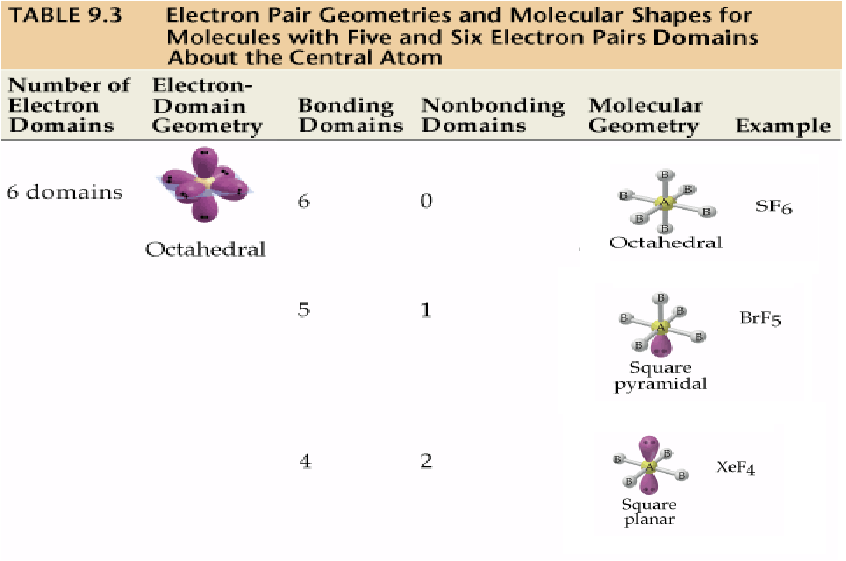
\includegraphics[scale=0.4]{molgeo6} \\

Usually an electron pair means a negative dipole, but sometimes geometry will cancel it out. See below:

\begin{tabular}{|c|c|c|}
\hline
EDs & Neutral & Polar \\ \hline
3 & trigonal planar & bent \\ \hline
4 & tetrahedral & trigonal planar, bent \\ \hline
5 & trigonal bipyramidal, linear & seesaw, T-shaped \\ \hline
6 & octahedral, square planar & square pyramidal\\ \hline
\end{tabular}
\section{Polarity}
\begin{tabular}{|c|c|}
\hline
$\Delta$EN & Polarity \\ \hline
[0, 0.5) & Non-polar covalent \\ \hline
[0.5, 1.7) & Polar covalent \\ \hline
1.7+ & Ionic \\ \hline
\end{tabular}

If the molecule turns out to be polar covalent, draw the appropriate charges $\delta\pm$ over the molecules, and the \emph{dipole moment} (arrow with $\delta+$ and $\delta-$ to indicate polarity direction) to the left of the molecule.
\chapter{Hybridization}
Valence bond theory says that bonds are formed by overlapping orbitals that contain shared electron pairs.

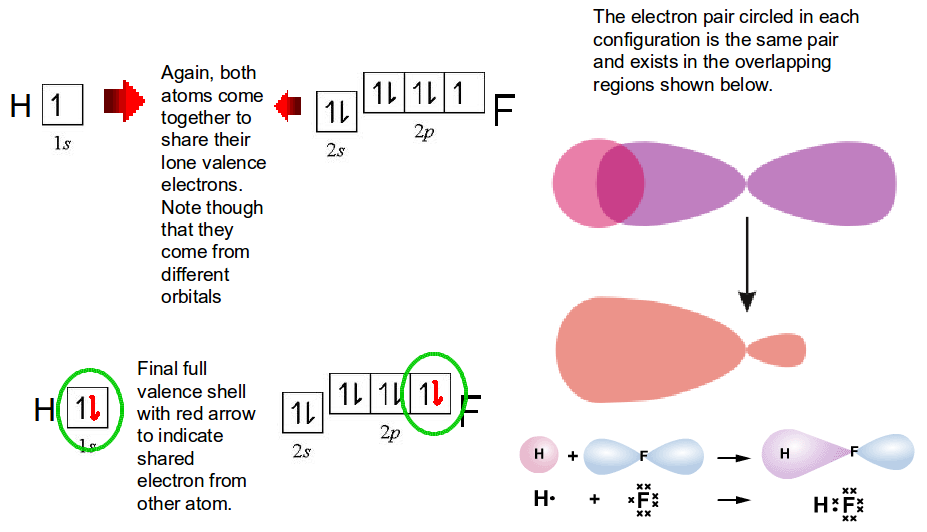
\includegraphics[scale=0.4]{hf} \\
See how the orbitals smush together into new shapes.

But the orbitals all looked the same in the electron geometry stuff! In truth, orbitals combine into identical \emph{hybrid orbitals}.

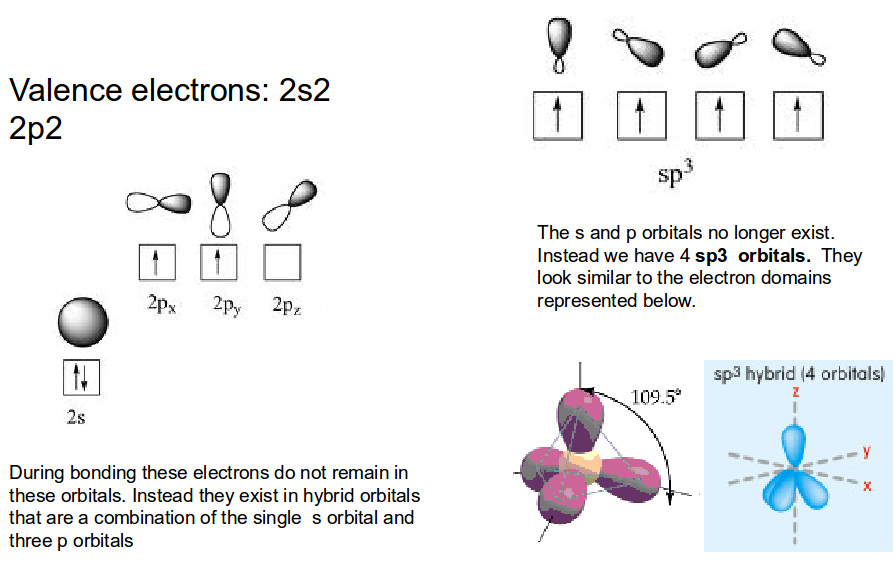
\includegraphics[scale=0.4]{mh4} \\

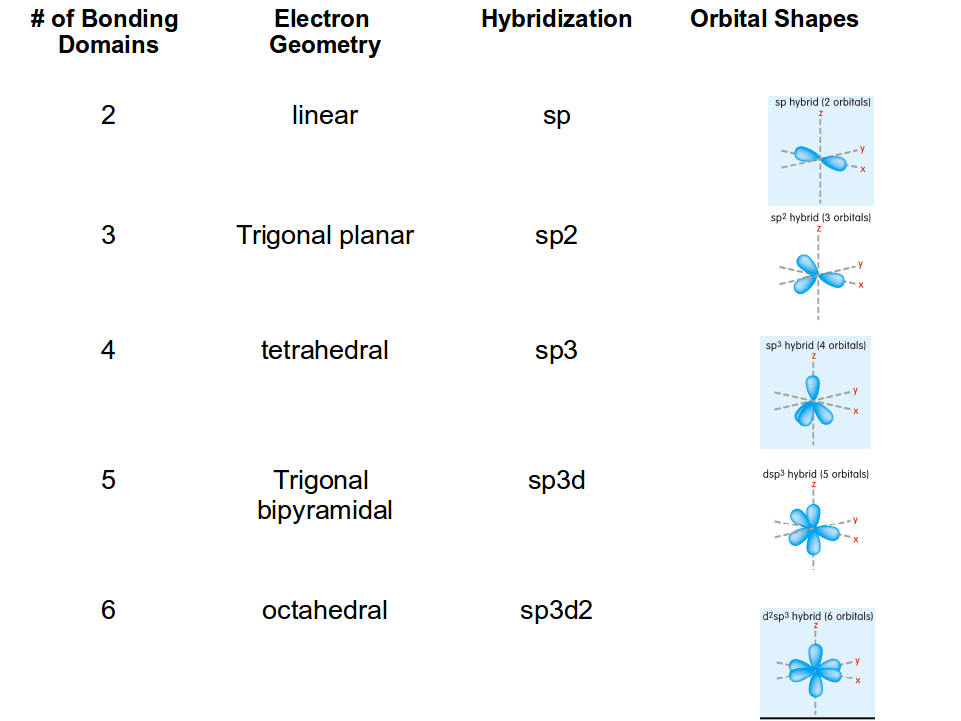
\includegraphics[scale=0.4]{hybridizationTable} \\

\section{Multiple bonds}
For each extra bond in a multiple (double/triple) bond, the number of available p-orbitals decreases.

So if there is a double bond, the p-orbitals only go up to 2.

If there is a triple bond, the p-orbitals only go up to 1.

For every overlap of hybridized orbitals (i.e. more than one bonding domain i.e. not hydrogen) a sigma $\sigma$ bond is created. 

For every overlap of p-orbitals a pi $\pi$ bond is created. 

\emph{In general, 1 bond is $\sigma$, and the rest are $\pi$.}

Say we have \ce{H-C#C-H}. The electron configuration of C is $1s^2 2s^2 2p^2$. C has 2 bonding domains, so it has \emph{sp} hybridized orbitals. There is a sigma bond between H and C, and between C and C: a total of 2 $\sigma$ bonds. The bond between the carbons is a triple bond, so less the sigma bond, there are 2 $\pi$ bonds.

Final word: the overlap of p-orbitals in multiple bonds makes the bonds much stronger.

\chapter{Intermolecular Forces}
\begin{description}
\item[Intramolecular forces] hold a molecule together e.g. bonds. Determine chemical properties e.g. reactivity. Stronger than intermolecular forces.
\item[Intermolecular forces] attract molecules to each other. Determine physical properties e.g. boiling point.
\end{description}
\section{London Dispersion Forces}
\begin{itemize}
	\item Between \emph{all molecules}
	\item Electrons randomly collect on one side of an atom, giving the atom a charge (\emph{instantaneous dipole}). Electrons in adjacent atoms are affected and also gain a charge (\emph{induced dipole}). 
	\item Though weak, happens frequently due to high speed
	\item \# of atoms, contact area, atomic radius $\uparrow$ LD $\uparrow$
	\item compactness $\uparrow$ LD $\downarrow$
	\item The smaller an atom, the closer the nucleus is to the valence electrons. A positive dipole, as it is attracted by a negative dipole, is also repelled by the nucleus.
	\item "polarizability": ability of electrons to move about and cause a charge
\end{itemize}	
\section{Dipole-dipole}
\begin{itemize}
\item Between \emph{polar substances}
\item Electrostatic attraction between oppositely charged sides of molecules
\end{itemize}
\section{Hydrogen bonding: a type of dipole-dipole}
\begin{itemize} 
\item \emph{Strongest}
\item Occurs in molecules containing \ce{H-O}, \ce{H-F}, \ce{H-N}
\end{itemize}
Stackability is a pretty good way to assess the strength of intermolecular forces. \\
\begin{tabular}{|c|c|c|p{2cm}|}
\hline
Name & Structure & BP& Reasoning \\ \hline
n-butanol & \chemfig{H-C(-[2]H)(-[6]H)-C(-[2]H)(-[6]H)-C(-[2]H)(-[6]H)-C(-[2]H)(-[6]H)-O(-[1]H)} & Highest & Good hydrogen bond location, large contact area \\ \hline
tertbutanol & \chemfig{C(-[2]C(-[0]H)(-[2]H)(-[4]H))(-[4]H)(-[6]C(-[0]H)(-[4]H)(-[6]H))-[,2]C(-[2]H)(-[6]H)-OH} & High & Better hydrogen bond location than the below \\ \hline
2-butanol & \chemfig{H-C(-[2]H)(-[6]H)-C(-[2]H)(-[6]H)-C(-[2]H)(-[6]O-[6]H)-C(-[2]H)(-[6]H)-H} & Lower & Worse hydrogen bond location \\ \hline
isobutanol & \chemfig{C(-[2]H)(-[4]H)(-[6]H)-[,2]C(-[2]C(-[0]H)(-[2]H)(-[4]H))(-[6]C(-[0]H)(-[4]H)(-[6]H))-OH} & Lowest & Contact area too little, bad hydrogen bond location \\ \hline
\end{tabular}

\end{document}
